% =============================================================================
\section{Nivel 1: moverse bien}
% =============================================================================

% ----------------------------------------------------------------------------- 1
\begin{frame}{Misión 1: la estrella del show}
  \begin{columns}[c]
    \column{0.5\textwidth}
    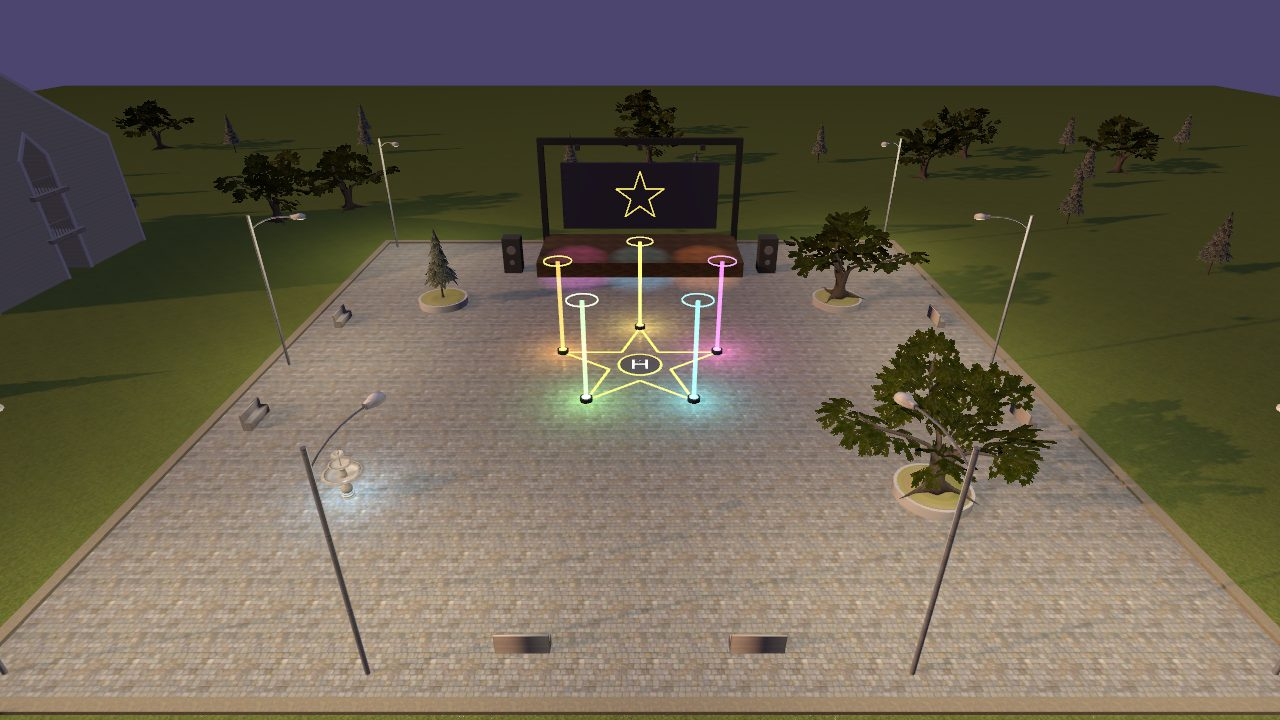
\includegraphics[width=\linewidth]{plaza_show}
    \column{0.47\textwidth}\small
    \textbf{Escenario}: una empresa de espectáculos quiere una estrella de 5 picos a 6 m de altura
    para el show de año nuevo.
    \begin{itemize}
      \item Mundo \cmd{plaza\_show}: la estrella dorada pintada en el piso.
      \item En cada pico, una baliza con un \textbf{aro a 6 m}: el dron tiene que pasar por adentro.
      \item \textbf{Viene de}: \cmd{square\_mission} (waypoints en offboard).
      \item \textbf{Lo nuevo}: los waypoints se \textbf{generan con una fórmula}.
    \end{itemize}
  \end{columns}
\end{frame}

\begin{frame}{La geometría de la estrella}
  \begin{columns}[c]
    \column{0.45\textwidth}\centering
    \begin{tikzpicture}[scale=0.42]
      \def\R{5} \def\r{1.91}
      \draw[gray!40] (0,0) circle (\R);
      \draw[gray!40,dashed] (0,0) circle (\r);
      \foreach \k in {0,...,4} {
        \pgfmathsetmacro{\a}{90-72*\k}
        \pgfmathsetmacro{\b}{90-72*\k-36}
        \coordinate (P\k) at (\a:\R);
        \coordinate (I\k) at (\b:\r);
      }
      \draw[naranja,thick] (P0)--(I0)--(P1)--(I1)--(P2)--(I2)--(P3)--(I3)--(P4)--(I4)--cycle;
      \foreach \k in {0,...,4} {\fill[azul] (P\k) circle (4pt); \fill[verde] (I\k) circle (3pt);}
      \node[above,font=\tiny] at (P0) {P0 (norte)};
      \node[right,font=\tiny] at (P1) {P1};
      \node[font=\tiny,right] at (I0) {I0};
      \draw[-{Stealth}] (0,0) -- (P0) node[midway,left,font=\tiny] {R};
      \fill (0,0) circle (2pt);
    \end{tikzpicture}
    \column{0.52\textwidth}\small
    \begin{itemize}
      \item \textbf{Picos} $P_k$: en el círculo de radio $R$, repartidos cada $360^\circ/N$, el primero
        al \textbf{norte}.
      \item \textbf{Interiores} $I_k$: en el círculo de radio $R\cdot$\cmd{inner\_ratio}, a medio
        camino (en ángulo) entre dos picos.
      \item Orden de vuelo: $P_0, I_0, P_1, I_1, \ldots$ y de vuelta a $P_0$.
      \item \cmd{inner\_ratio = 0.382}: estrella regular de 5.\\
        \cmd{inner\_ratio = 0}: polígono. Con \cmd{points:=4} debe salir \textbf{un cuadrado}.
    \end{itemize}
  \end{columns}
\end{frame}

\begin{frame}{Un punto en polares, en NED}
  \begin{columns}[c]
    \column{0.45\textwidth}\centering
    \begin{tikzpicture}[scale=1.1]
      \draw[-{Stealth},verde] (0,0) -- (0,2.2) node[above,font=\scriptsize] {N (x)};
      \draw[-{Stealth},rojo] (0,0) -- (2.2,0) node[right,font=\scriptsize] {E (y)};
      \draw[thick,azul] (0,0) -- (55:1.9);
      \fill[azul] (55:1.9) circle (2pt);
      \draw[-{Stealth}] (0,0.7) arc (90:55:0.7);
      \node[font=\scriptsize] at (0.45,0.95) {$a$};
      \node[font=\scriptsize,azul] at (1.6,1.75) {$(r\cos a,\ r\sin a)$};
    \end{tikzpicture}
    \column{0.52\textwidth}\small
    Con el ángulo $a$ medido \textbf{desde el norte, hacia el este}:
    \[ \text{norte} = r\cos a \qquad \text{este} = r\sin a \]
    \begin{ojo}
      \small Es al revés de la trigonometría de la escuela (desde el eje x, antihorario). Aquí
      $a = 0$ es el norte y $a = 90^\circ$ el este, porque así mide PX4 el yaw.
    \end{ojo}
  \end{columns}
\end{frame}

\begin{frame}[fragile]{Tu parte: \texttt{vertices()}}
  \begin{lstlisting}[style=cpp,caption={Lo que trae el reto (estrella\_show.cpp)}]
std::vector<Point> vertices() const {
  std::vector<Point> out;
  const float z = static_cast<float>(-altitude_);
  // TODO 1: los picos. Hay points_ picos repartidos en 360°, el primero al
  //   norte. ... Pista: el ángulo del pico k es 2*pi*k / points_ (en radianes).
  // TODO 2: los vértices interiores. Si inner_ratio_ > 0, después de cada
  //   pico va un vértice a radio radius_ * inner_ratio_, ...
  // Para agregar un punto:  out.push_back({norte, este, z});
  return out;
}
  \end{lstlisting}
  \small Si \cmd{vertices()} regresa la lista vacía, el nodo despega, avisa y aterriza.
\end{frame}

\begin{frame}{Cómo vuela y cómo se califica}
  \begin{columns}[c]
    \column{0.5\textwidth}
    \begin{tikzpicture}[node distance=0.35cm,st/.style={draw=azul,fill=azulclaro,rounded corners,font=\tiny,minimum width=1.4cm}]
      \node[st] (a) {WARMUP}; \node[st,below=of a] (b) {TAKEOFF};
      \node[st,below=of b,fill=yellow!20] (c) {STAR};
      \node[st,below=of c] (d) {CENTER}; \node[st,below=of d] (e) {LANDING};
      \draw[-{Stealth}] (a)--(b); \draw[-{Stealth}] (b)--node[right,font=\tiny]{al centro, a 6 m}(c);
      \draw[-{Stealth}] (c)--node[right,font=\tiny]{último vértice}(d); \draw[-{Stealth}] (d)--(e);
      \draw[-{Stealth}] (c.west) to[bend left=60] node[left,font=\tiny,align=right]{a \textless0.5 m:\\0.5 s quieto,\\siguiente} (c.west|-c.north);
    \end{tikzpicture}
    \column{0.47\textwidth}
    \begin{terminal}{al aterrizar}
Qué tan cerca pasó de cada vértice:\\
\ \ 1: 0.15 m OK\\
\ \ 2: 0.11 m OK\\
\ \ ...\\
\ 11: 0.05 m OK\\
Misión cumplida
    \end{terminal}
    \small\textbf{Éxito}: pasa a menos de \cmd{tolerance} (0.5 m) de cada vértice, regresa al centro y aterriza.
  \end{columns}
\end{frame}

\begin{frame}{Errores típicos en la misión 1}
  \begin{itemize}\small
    \item \textbf{Radianes vs grados}: \cmd{std::cos} recibe radianes. $2\pi k/N$, no $360k/N$.
    \item \textbf{División entera}: \cmd{2 * M\_PI * k / points\_} está bien; \cmd{k / points\_ * 2 * M\_PI} da 0
      (\cmd{k} y \cmd{points\_} son enteros).
    \item \textbf{double a float}: \cmd{Point} es \cmd{std::array<float,3>}; usen \cmd{static\_cast<float>()}.
    \item \textbf{Cerrar la figura}: el último punto debe ser otra vez el pico 0.
    \item \textbf{z positiva}: si el dron se va al suelo, les faltó el signo menos.
  \end{itemize}
  \begin{idea}
    \small Prueben \cmd{points:=6}, \cmd{points:=4 inner\_ratio:=0.0} (cuadrado) y \cmd{radius:=3.0}:
    un buen generador funciona para cualquier N.
  \end{idea}
\end{frame}

% ----------------------------------------------------------------------------- 2
\begin{frame}{Misión 2: inspección de un pilar}
  \begin{columns}[c]
    \column{0.5\textwidth}
    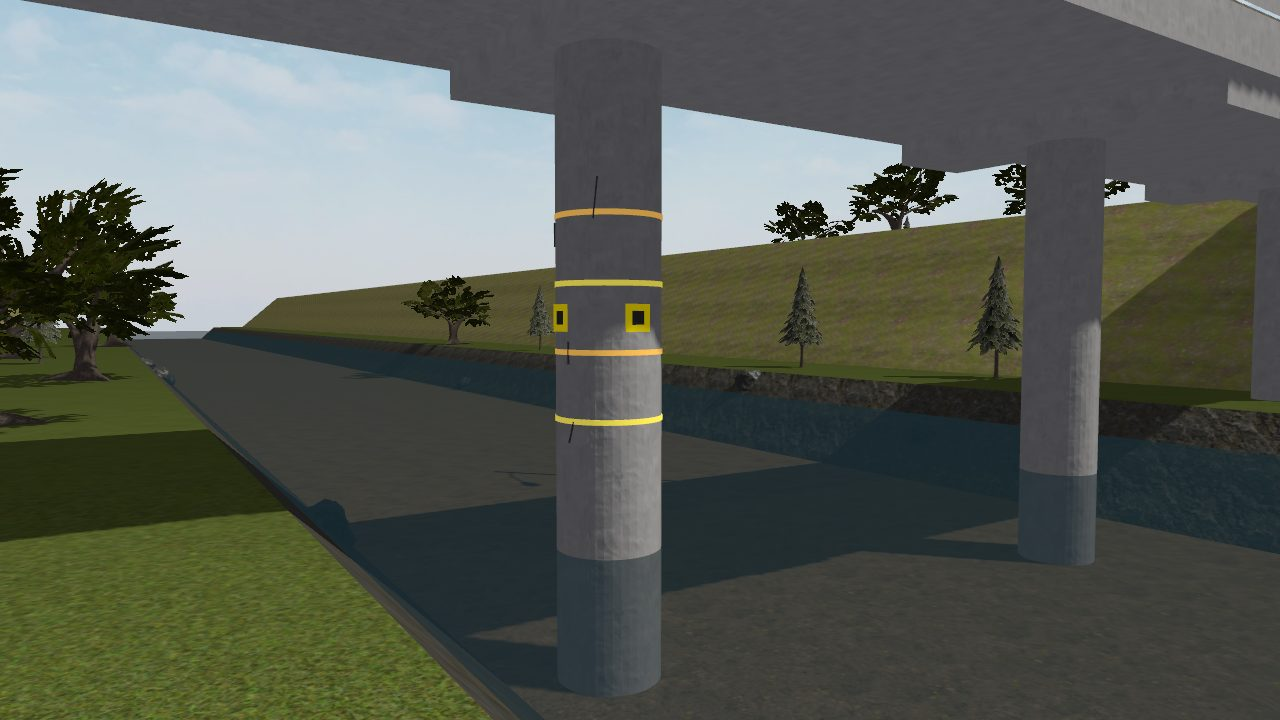
\includegraphics[width=\linewidth]{puente_rio_pilar}
    \column{0.47\textwidth}\small
    \textbf{Escenario}: una constructora necesita fotos de un pilar de puente desde todos los
    ángulos y alturas.
    \begin{itemize}
      \item Subir en \textbf{hélice} alrededor del pilar: 3 vueltas de 1 m a 4 m.
      \item La nariz (la cámara) \textbf{siempre apuntando al pilar}.
      \item \textbf{Viene de}: \cmd{orbit\_mission} + \cmd{figure\_eight}.
      \item Las bandas de colores del pilar están justo a 1, 2, 3 y 4 m.
    \end{itemize}
  \end{columns}
\end{frame}

\begin{frame}{La hélice: un círculo que sube}
  \begin{columns}[c]
    \column{0.45\textwidth}\centering
    \begin{tikzpicture}[scale=0.85]
      \draw[thick,fill=gray!30] (-0.25,0) rectangle (0.25,3.2);
      \draw[azul,thick,domain=0:1080,samples=200,smooth,variable=\t]
        plot ({1.3*cos(\t)}, {0.3+0.0024*\t + 0.25*sin(\t)});
      \node[font=\tiny,right] at (1.4,0.3) {1 m: entra};
      \node[font=\tiny,right] at (1.4,2.9) {4 m: sale};
      \draw[-{Stealth},dashed] (0,-0.3) -- (1.3,-0.3) node[midway,below,font=\tiny] {radio 3 m};
    \end{tikzpicture}
    \column{0.52\textwidth}\small
    Con velocidad angular $\omega = v/R$ y empezando en el ángulo $\theta_0$:
    \[ \theta(t) = \theta_0 + \omega t \]
    \[ N(t) = N_c + R\cos\theta(t) \qquad E(t) = E_c + R\sin\theta(t) \]
    y la altura \textbf{sube lineal} de \cmd{z\_start} a \cmd{z\_end} en la duración total
    $T = \text{vueltas}\cdot 2\pi R / v$.
    \vspace{0.3em}

    \footnotesize $\theta_0$ es el punto del círculo más cercano al despegue: así llega sin rodear el pilar.
  \end{columns}
\end{frame}

\begin{frame}{Derivar para el feedforward}
  \small \cmd{figure\_eight} ya lo hace con su curva: la velocidad es la derivada de la posición.
  Para un círculo:
  \[
    \frac{d}{dt}\bigl(R\cos\theta(t)\bigr) = -R\,\omega\sin\theta(t)
    \qquad
    \frac{d}{dt}\bigl(R\sin\theta(t)\bigr) = R\,\omega\cos\theta(t)
  \]
  \begin{columns}[c]
    \column{0.55\textwidth}
    \begin{itemize}
      \item La velocidad es \textbf{tangente} al círculo, de magnitud $R\omega = v$.
      \item La aceleración (segunda derivada) apunta \textbf{al centro}, de magnitud $R\omega^2$.
      \item Y en $z$: si sube lineal, ¿cuánto vale $dz/dt$? (cuidado: NED, arriba es $-z$).
    \end{itemize}
    \column{0.42\textwidth}
    \begin{tikzpicture}[scale=0.8]
      \draw[gray] (0,0) circle (1.4);
      \fill (40:1.4) circle (2pt);
      \draw[-{Stealth},azul,thick] (40:1.4) -- ++(130:0.9) node[above,font=\tiny] {$v$};
      \draw[-{Stealth},rojo,thick] (40:1.4) -- (40:0.6) node[below,font=\tiny] {$a$};
      \fill (0,0) circle (1.5pt);
    \end{tikzpicture}
  \end{columns}
\end{frame}

\begin{frame}{Apuntar al pilar}
  \begin{columns}[c]
    \column{0.45\textwidth}\centering
    \begin{tikzpicture}[scale=0.9]
      \draw[gray] (0,0) circle (1.5);
      \fill[gray!60] (0,0) circle (0.3);
      \fill[azul] (130:1.5) circle (3pt);
      \draw[-{Stealth},thick,naranja] (130:1.5) -- (130:0.4) node[midway,above,font=\tiny,sloped] {nariz};
      \draw[-{Stealth},verde] (0,0) -- (0,2) node[above,font=\tiny] {N};
      \draw[-{Stealth},rojo] (0,0) -- (2,0) node[right,font=\tiny] {E};
    \end{tikzpicture}
    \column{0.52\textwidth}\small
    El yaw que apunta del dron al centro es el ángulo del vector \emph{dron $\rightarrow$ centro}:
    \[ \psi = \operatorname{atan2}(E_c - E,\ N_c - N) \]
    (\cmd{atan2(este, norte)}: el orden importa).
    \vspace{0.3em}

    Y \cmd{yawspeed} = qué tan rápido gira esa dirección: en un círculo, lo mismo que $\omega$.
  \end{columns}
\end{frame}

\begin{frame}{Cómo se califica la hélice}
  \small Mientras vuela, el nodo mide contra la \textbf{posición real} (no contra el setpoint):
  \begin{columns}[c]
    \column{0.55\textwidth}
    \begin{itemize}
      \item \textbf{Radio}: distancia real al eje del pilar, dentro de $3 \pm 0.3$ m.
      \item \textbf{Yaw}: la nariz contra la dirección real al pilar, error $< 10^\circ$.
      \item \textbf{Vueltas}: suma del ángulo recorrido alrededor del pilar $\geq$ 90\% de 3.
      \item \textbf{Altura}: llegó a \cmd{z\_end} (4 m) $- 0.3$.
    \end{itemize}
    \column{0.42\textwidth}
    \begin{terminal}{al aterrizar}
vueltas: 2.99 de 3.00 OK\\
altura máxima: 3.99 m OK\\
error de radio: 0.11 m OK\\
error de yaw: 6.1° OK\\
Misión cumplida
    \end{terminal}
  \end{columns}
\end{frame}

\begin{frame}{El extra: arrancar suave}
  \begin{columns}[c]
    \column{0.55\textwidth}\small
    Si todo pasa menos el yaw, que se pasa de 10° \textbf{justo al empezar}:
    \begin{itemize}
      \item En $t = 0$ la velocidad del setpoint salta de 0 a $v$ en un instante.
      \item El dron no puede acelerar infinito: se queda atrás un momento.
      \item El setpoint ya va adelante y la nariz apunta a donde \emph{debería} estar, no a donde está.
    \end{itemize}
    Pista: que la velocidad suba de 0 a $v$ en 1--2 s (y no olviden sumar ese tiempo a la duración).
    \column{0.42\textwidth}
    \begin{tikzpicture}[x=0.6cm,y=0.9cm]
      \draw[-{Stealth}] (0,0) -- (5.5,0) node[right,font=\tiny] {t};
      \draw[-{Stealth}] (0,0) -- (0,1.6) node[above,font=\tiny] {v};
      \draw[rojo,thick] (0,0) -- (0,1.2) -- (5,1.2);
      \draw[verde,thick,domain=0:5,samples=40] plot (\x,{1.2*(1-exp(-\x/0.8))});
      \node[font=\tiny,rojo] at (3.3,1.4) {escalón};
      \node[font=\tiny,verde] at (3.3,0.8) {rampa};
    \end{tikzpicture}
  \end{columns}
\end{frame}

% ----------------------------------------------------------------------------- 3
\begin{frame}{Misión 3: entrega a domicilio}
  \begin{columns}[c]
    \column{0.5\textwidth}
    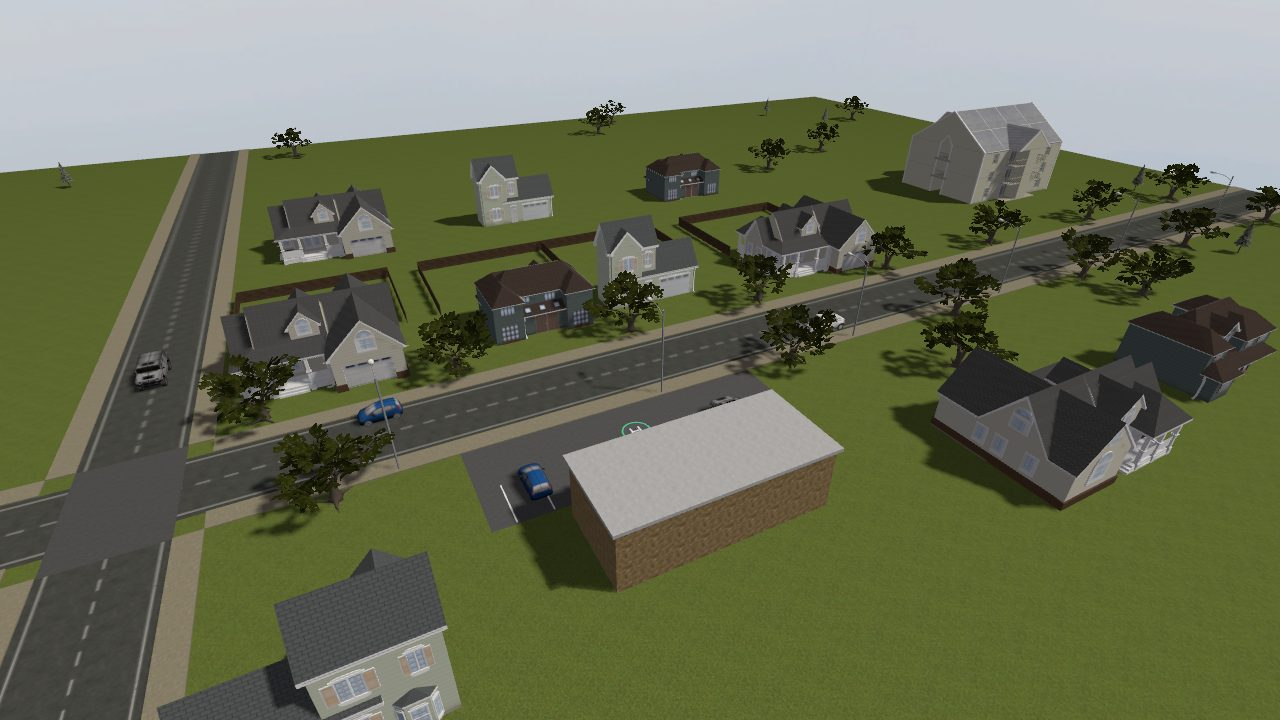
\includegraphics[width=\linewidth]{barrio_entrega}
    \column{0.47\textwidth}\small
    \textbf{Escenario}: llevar un medicamento de la farmacia a una casa a \textasciitilde40 m,
    dejarlo y volver solo.
    \begin{itemize}
      \item \textbf{Sin offboard}: PX4 vuela cada tramo con sus modos; el nodo solo decide qué sigue.
      \item Si el nodo se muere, el dron se queda en Hold (no hay failsafe de offboard).
      \item \textbf{Viene de}: \cmd{goto\_mission} + \cmd{return\_home} + \cmd{set\_home}.
    \end{itemize}
  \end{columns}
\end{frame}

\begin{frame}{Las fases (el log las numera [1/9] \ldots{} [9/9])}
  \centering
  \begin{tikzpicture}[node distance=0.25cm,st/.style={draw=azul,fill=azulclaro,rounded corners,font=\tiny,minimum width=1.8cm,minimum height=0.45cm,align=center}]
    \node[st] (1) {WAIT\_GPS};
    \node[st,right=of 1] (2) {ARMING};
    \node[st,right=of 2] (3) {TAKEOFF};
    \node[st,right=of 3] (4) {FLY};
    \node[st,right=of 4] (5) {LAND\_DEST};
    \node[st,below=0.9cm of 5,fill=yellow!20] (6) {DELIVER};
    \node[st,left=of 6,fill=yellow!20] (7) {REARM};
    \node[st,left=of 7,fill=yellow!20] (8) {TAKEOFF\_BACK};
    \node[st,left=of 8,fill=yellow!20] (9) {SET\_HOME};
    \node[st,left=of 9,fill=yellow!20] (10) {RETURN};
    \foreach \a/\b in {1/2,2/3,3/4,4/5,5/6,6/7,7/8,8/9,9/10} \draw[-{Stealth}] (\a) -- (\b);
  \end{tikzpicture}
  \vspace{0.5em}
  \begin{columns}[t]
    \column{0.5\textwidth}\small
    \textbf{Ya funciona}: de la farmacia hasta aterrizar en el patio (azul).
    \column{0.47\textwidth}\small
    \textbf{Tu parte} (amarillo): esperar desarmado, volver a armar y despegar, \textbf{arreglar casa}
    y regresar con Return.
  \end{columns}
\end{frame}

\begin{frame}[fragile]{Las ayudas que ya están hechas}
  \begin{lstlisting}[style=cpp,caption={entrega\_domicilio: tu trabajo es decidir CUÁNDO llamar cada una}]
bool arm_when_ready();        // Hold y armar, reintentando cada 1 s; true si ya armó
void take_off();              // NAV_TAKEOFF sobre donde está, a cruise_alt
void go_to_target();          // DO_REPOSITION al patio: vuela y queda en Hold
void set_home_to_pharmacy();  // DO_SET_HOME con las coordenadas de la farmacia
bool at_cruise_alt() const;   // en Hold y a la altura de crucero
double home_offset() const;   // qué tan lejos de la farmacia está "casa"
  \end{lstlisting}
  \small Y \cmd{px4\_.home().update\_count}: sube cada vez que PX4 mueve ``casa''
  (así sabes que aceptó el \cmd{DO\_SET\_HOME}, como en \cmd{set\_home.cpp}).
\end{frame}

\begin{frame}{La trampa: ¿dónde quedó casa?}
  \begin{columns}[c]
    \column{0.5\textwidth}\small
    PX4 fija ``casa'' \textbf{donde arma}.
    \begin{enumerate}
      \item Arma en la farmacia $\Rightarrow$ casa = farmacia.
      \item Aterriza en el patio y desarma.
      \item \textbf{Vuelve a armar en el patio} $\Rightarrow$ casa = \ldots
    \end{enumerate}
    Si mandan Return así, ¿a dónde regresa?
    \vspace{0.3em}
    \begin{idea}
      \small El nodo guarda las coordenadas de la farmacia al principio
      (\cmd{pharmacy\_lat\_}, \cmd{pharmacy\_lon\_}). \cmd{px4\_.home()} les dice dónde cree PX4
      que está casa.
    \end{idea}
    \column{0.47\textwidth}
    \begin{tikzpicture}[scale=0.8]
      \node[draw,fill=green!20,font=\tiny] (f) at (0,0) {farmacia (H)};
      \node[draw,fill=orange!30,font=\tiny] (p) at (3,3) {patio};
      \draw[-{Stealth},thick,azul] (f) to[bend left] node[above left,font=\tiny] {ida} (p);
      \draw[-{Stealth},thick,verde,dashed] (p) to[bend left] node[below right,font=\tiny] {Return correcto} (f);
      \draw[-{Stealth},thick,rojo] (p.east) .. controls (4.6,3.6) and (4.2,2.2) .. node[right,font=\tiny] {Return con casa en el patio} (p.south east);
    \end{tikzpicture}
  \end{columns}
\end{frame}

\begin{frame}{Alturas y GPS en la entrega}
  \small
  \begin{itemize}
    \item La plataforma está en \textbf{lat 47.3982949, lon 8.5463757} (36 m N, 16 m E de la farmacia).
    \item La ruta directa pasa \textbf{sobre la casa destino}, de \textasciitilde9 m: \cmd{cruise\_alt}
      tiene que librarla (15 m por defecto).
    \item Los comandos piden altura \textbf{AMSL} (sobre el nivel del mar): el nodo guarda la altura del
      suelo al principio y le suma \cmd{cruise\_alt}.
    \item \cmd{Return} sube primero a \cmd{RTL\_RETURN\_ALT} (30 m en el x500 de SITL), vuela a casa y baja.
  \end{itemize}
  \begin{terminal}{al aterrizar en la farmacia}
De vuelta en la farmacia y desarmado. Misión de 119 s\\
\ \ a 0.01 m de la H OK\\
Misión cumplida
  \end{terminal}
\end{frame}
